\documentclass[sigplan,review]{acmart}
\usepackage{tikz}
\setcopyright{none}

\begin{document}
\title{Making CRDTs Byzantine Fault Tolerant}
\author{Martin Kleppmann}
\email{martin@kleppmann.com}
\orcid{0000-0001-7252-6958}
\affiliation{%
  \institution{University of Cambridge}
  \streetaddress{William Gates Building, JJ Thomson Avenue}
  \city{Cambridge}
  \country{UK}
  \postcode{CB3 0FD}
}

\begin{abstract}
It is often claimed that CRDTs ensure consistency of replicated data in peer-to-peer systems.
However, peer-to-peer systems usually consist of untrusted nodes that may deviate from the specified protocol (i.e.\ exhibit Byzantine faults), and most existing CRDT algorithms cannot guarantee consistency in the presence of such faults.
This paper shows how to adapt existing non-Byzantine CRDT algorithms and make them Byzantine fault-tolerant.
The proposed scheme can tolerate any number of Byzantine nodes (making it immune to Sybil attacks), guarantees Strong Eventual Consistency, and requires only modest changes to existing CRDT algorithms.
\end{abstract}

\begin{CCSXML}
<ccs2012>
    <concept>
        <concept_id>10010520.10010521.10010537.10010540</concept_id>
        <concept_desc>Computer systems organization~Peer-to-peer architectures</concept_desc>
        <concept_significance>500</concept_significance>
    </concept>
    <concept>
        <concept_id>10002978.10003006.10003013</concept_id>
        <concept_desc>Security and privacy~Distributed systems security</concept_desc>
        <concept_significance>300</concept_significance>
    </concept>
</ccs2012>
\end{CCSXML}

\ccsdesc[500]{Computer systems organization~Peer-to-peer architectures}
\ccsdesc[300]{Security and privacy~Distributed systems security}

\keywords{Byzantine fault tolerance, CRDTs, optimistic replication, eventual consistency}
\maketitle

\section{Introduction}\label{sec:introduction}

A key characteristic of many peer-to-peer (P2P) systems is that peers are not under the control of a single authority~\cite{Buford:2010}; indeed, many P2P applications are \emph{open, trustless} systems in which anybody on the Internet can run a node and join the system.
As the operators of nodes cannot be trusted, it must be assumed that some nodes may not correctly follow the specified protocol of the network: be it due to bugs in implementations, deliberate attempts to gain an advantage over other nodes, or sheer vandalism, a P2P system cannot rely on nodes always behaving the way that the designers of the system intended.
Nodes may send false or contradictory messages to other nodes, and they may try to actively undermine any guarantees the system aims to provide.

When a node deviates from the specified protocol, we call it \emph{Byzantine-faulty} (or simply \emph{Byzantine}), regardless of whether the deviation is by accident or by malice~\cite{Lamport:1982}.
Byzantine behaviour is not always detectable by other nodes, since a Byzantine node may attempt to hide its protocol violations.
One approach would be to try to identify Byzantine nodes and exclude them from the system, but this is unlikely to be effective if the banned node can simply rejoin the system under a different identity.
A more robust approach is to \emph{tolerate} Byzantine faults: that is, to ensure that the system can meet its advertised guarantees even when some of its nodes are Byzantine-faulty.

Conflict-free Replicated Data Types (CRDTs)~\cite{Shapiro:2011} are often presented as an approach for providing consistency of replicated data in peer-to-peer systems~\cite{vanderLinde:2017fu,Weiss:2009ht,Nicolaescu:2016}, because they do not require a central server for concurrency control.
However, despite ostensibly targeting P2P systems, the vast majority of CRDT algorithms actually do not tolerate Byzantine faults, since they assume that all participating nodes correctly follow the protocol.
If such algorithms are deployed in a system with Byzantine nodes, the algorithm cannot guarantee the consistency properties that CRDTs are supposed to provide, and nodes may end up with permanently inconsistent replicas of the shared data.

In some circumstances, the lack of Byzantine fault tolerance can be justified by restricting CRDT-based collaboration to small, trusted groups of nodes: for example, in a collaborative editor, the set of users who are authorised to edit a document may be limited to immediate colleagues, who may trust each other to run the CRDT algorithm correctly.
However, as the range of collaborators is widened to public settings such as wikis~\cite{Nedelec:2016eo,Weiss:2007,Weiss:2009ht}, and as CRDT designers seek to enable collaboration at ``massive scale''~\cite{Andre:2013,Weiss:2009ht,Lv:2016}, blindly trusting collaborators to do everything correctly seems like an increasingly dangerous assumption.

Fortunately, it is possible to retrofit Byzantine fault tolerance to some CRDTs without having to redesign them from scratch.
This paper introduces some general-purpose principles that can be used to make operation-based CRDT algorithms robust against Byzantine faults.

\section{Background and system model}\label{sec:background}

This section highlights some of the problems that CRDT algorithms encounter when faced with Byzantine faults.

\subsection{Nodes and network links}\label{sec:system-model}

This paper assumes a peer-to-peer system in which all nodes are equal, and in which nodes can communicate by exchanging messages over pairwise network links.
The network is not necessarily complete, i.e.\ it is not required for every node to be able to communicate with every other node.
Nodes and network links are assumed to be asynchronous and unreliable, so messages may be lost.
However, we can assume that network links are authenticated (e.g. using cryptographic signatures), so that a node is able to reliably determine which remote node it is communicating with.

Many papers on Byzantine fault tolerance assume that no more than some upper bound of nodes is Byzantine (a common assumption is that there are $3f+1$ nodes in the system, and that no more than $f$ of them are Byzantine).
This assumption is problematic for P2P systems, since it necessitates centralised control over which nodes are allowed to join the network~-- otherwise many adversary-controlled nodes could join the network and overwhelm it, which is known as a Sybil attack~\cite{Douceur:2002}.

In contrast, this paper makes no such assumption about the number of Byzantine nodes: it is possible to guarantee the correctness of CRDTs even in systems in which \emph{arbitrarily many} nodes are Byzantine, e.g.\ where the Byzantine nodes outnumber the correct nodes.
This is possible because CRDT-based applications are \emph{invariant confluent}, as explained in prior work~\cite{BECPreprint}.
The algorithms developed in this paper can therefore safely be used in open P2P systems that anybody can join, without requiring expensive Sybil countermeasures such as proof-of-work~\cite{Nakamoto:2008}.

\begin{figure*}
\centering
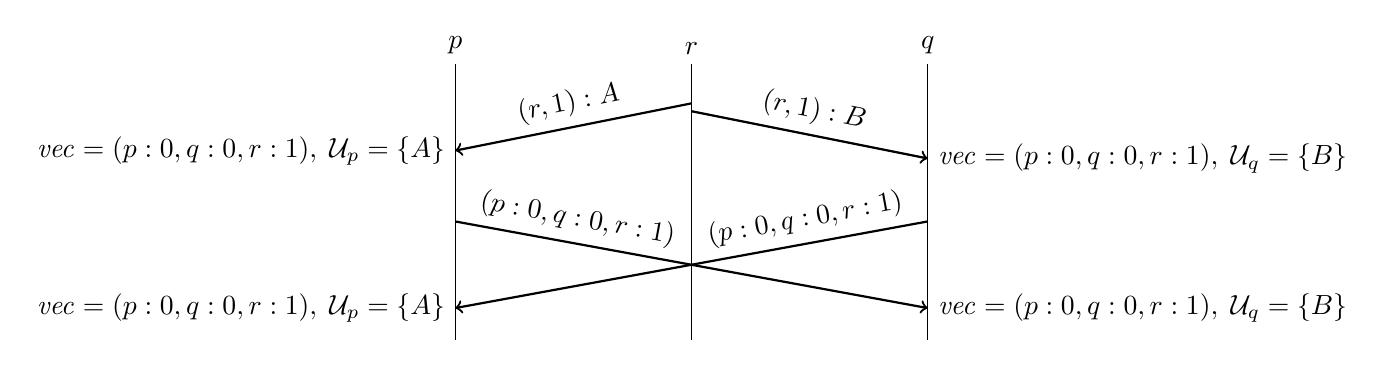
\begin{tikzpicture}
\draw (0, 0.5) node [above] {$p$} -- (0, -3);
\draw (3, 0.5) node [above] {$r$} -- (3, -3);
\draw (6, 0.5) node [above] {$q$} -- (6, -3);
\draw[thick,->] (3, 0) to node [above,sloped] {$(r, 1): A$} (0, -0.6) node [left] {$\mathit{vec} = (p:0,q:0,r:1),\; \mathcal{U}_p = \{A\}$};
\draw[thick,->] (3, -0.1) to node [above,sloped] {$(r, 1): B$} (6, -0.7) node [right] {$\mathit{vec} = (p:0,q:0,r:1),\; \mathcal{U}_q = \{B\}$};
\draw[thick,->] (0, -1.5) to node [above,pos=0.25,sloped] {$(p:0,q:0,r:1)$} (6, -2.6) node [right] {$\mathit{vec} = (p:0,q:0,r:1),\; \mathcal{U}_q = \{B\}$};
\draw[thick,->] (6, -1.5) to node [above,pos=0.25,sloped] {$(p:0,q:0,r:1)$} (0, -2.6) node [left] {$\mathit{vec} = (p:0,q:0,r:1),\; \mathcal{U}_p = \{A\}$};
\end{tikzpicture}
\caption{Byzantine node $r$ sends two different updates ($A$ and $B$) with the same ID $(r,1)$ to correct nodes $p$ and $q$. Now, $p$ and $q$ have identical vector clocks, even though they have delivered different sets of updates $\mathcal{U}_p \ne \mathcal{U}_q$.}
\label{fig:vectorclocks}
\end{figure*}

\subsection{Correctness of CRDTs}\label{sec:sec}

The standard model of correctness for CRDTs is Strong Eventual Consistency~\cite{Shapiro:2011,Gomes:2017gy}, which requires:
\begin{description}
\item[Eventual delivery:] An update delivered at a correct replica is eventually delivered at all correct replicas.
\item[Convergence:] Correct replicas that have delivered the same set of updates (possibly in a different order) have equivalent state.
\item[Termination:] All method executions terminate.
\end{description}
A replica (or node) is \emph{correct} if it is not faulty.

Termination is generally easy to ensure, so we focus on the other two properties.
Systems usually ensure eventual delivery by using a reliable broadcast protocol, such as a gossip protocol~\cite{Leitao:2009fi}, to disseminate updates.
To ensure convergence, operation-based CRDTs construct updates such that they are commutative: delivering them in any order results in the same replica state.
In some cases, a causal delivery algorithm additionally ensures that when one update has a dependency on an earlier update, the earlier update is delivered before the later update on all replicas.

\subsection{Eventual delivery with Byzantine nodes}\label{sec:delivery}

In a non-Byzantine system, eventual delivery can obviously only be achieved if there is some way for every pair of correct nodes to communicate, either directly or indirectly via other correct nodes.
Two nodes that are permanently partitioned from each other can never communicate and hence cannot deliver the same updates.

This idea generalises to Byzantine systems: if $p$ and $q$ are correct nodes, and if all of the communication paths between $p$ and $q$ go via Byzantine nodes, then eventual delivery cannot be guaranteed, since the Byzantine nodes may choose to block communication between $p$ and $q$.
To ensure eventual delivery, we therefore have to assume that any two correct nodes can communicate either directly, or indirectly via other correct (non-Byzantine) nodes.

We focus on the case where two correct nodes $p$ and $q$ can communicate with each other directly; the case of indirect communication via other correct nodes then consists simply of several instances of such pairwise direct communication, chained together.
Eventual delivery then requires that if $p$ has delivered some update $u$, then $q$ must also eventually deliver $u$.

To ensure that $p$ and $q$ eventually deliver the same set of updates, a simple but inefficient algorithm would be: periodically, $p$ sends $q$ every update that it has not already received from $q$, and vice versa.
This algorithm has the downside that for every update it has ever received, a node needs to keep track of which nodes have seen the update.
The advantage of this algorithm is that it is robust against Byzantine nodes: regardless of whether an update originated from a Byzantine or non-Byzantine node, correct nodes will propagate it to other correct nodes.

\subsubsection{Vector clocks}\label{sec:vector-clocks}

It would be desirable to have a more efficient protocol for nodes $p$ and $q$ to determine which updates they need to exchange so that, at the end, both have delivered the same set of updates (an \emph{anti-entropy} or \emph{reconciliation} protocol).
A common algorithm for this purpose is to use \emph{vector clocks}: each node sequentially numbers the updates that it generates, and so the set of updates that a node has delivered can be summarised by remembering just the highest sequence number from each node.

Unfortunately, vector clocks are not safe in the presence of Byzantine nodes, as shown in Figure~\ref{fig:vectorclocks}.
This is because a Byzantine node may generate several distinct updates with the same sequence number, and send them to different nodes.
Subsequently, when correct nodes $p$ and $q$ exchange vector clocks, they may believe that they have delivered the same set of updates because their vector clocks are identical, even though they have in fact delivered different updates.

Even if updates are signed, this type of misbehaviour by Byzantine nodes cannot be ruled out.
The reuse of the same sequence number might later be detected, but this would require an additional protocol on top of vector clocks.

\subsection{Convergence with Byzantine nodes}\label{sec:convergence}

Achieving the convergence property of Strong Eventual Consistency depends on the state update logic that a CRDT algorithm executes when an update is delivered.
We can assume that correct nodes all execute the same update logic, but Byzantine nodes may send arbitrarily malformed updates to the correct nodes.

Some types of updates can easily be identified as malformed and rejected, for example because they do not follow the message structure expected by the CRDT algorithm.
If the decision whether to reject an update is a deterministic function of the update itself, and does not depend on the state of the delivering node, then it is easy to ensure convergence, since all correct nodes will make the same decision on whether to reject a given update.

More problematic are updates that may or may not be valid, depending on the replica state of the node delivering the update.
To give a few examples:
\begin{itemize}
\item Many CRDTs assign a unique identifier to each item (e.g.\ each element in a sequence); the data structure does not allow multiple items with the same ID, since then an ID would be ambiguous.
Say a Byzantine node generates two different updates $u_1$ and $u_2$ that create two different items with the same ID.
If a node has already delivered $u_1$ and then subsequently delivers $u_2$, the update $u_2$ will be rejected, but a node that has not previously delivered $u_1$ may accept $u_2$.
Since one node accepted $u_2$ and the other rejected it, those nodes fail to converge, even if we have eventual delivery.

\item In many CRDTs, one operation depends on a prior one: for example, an element in a sequence can only be deleted if that element was previously inserted, but a nonexistent element cannot be deleted.
With non-Byzantine nodes, the metadata on updates can ensure that causally prior updates are delivered before causally later ones, but Byzantine nodes may not set this metadata correctly.
Consequently, if update $u_2$ depends on update $u_1$, it could happen that some nodes deliver $u_1$ before $u_2$ and hence process both updates correctly, but other nodes may try to deliver $u_2$ and fail because they have not yet delivered $u_1$.
This situation also leads to divergence.

\item Some CRDTs include values in an update that must be computed in a certain way.
For example, in WOOT~\cite{Oster:2006} and YATA~\cite{Nicolaescu:2016}, an insertion operation must reference the IDs of the predecessor and successor elements, and the algorithms depend on the predecessor appearing before the successor in the sequence.
The order of these elements is not apparent from the IDs alone, so the algorithm must inspect the CRDT state to check that the predecessor and successor references are valid.
\end{itemize}

\section{Tolerating Byzantine faults}\label{sec:solution}

To achieve Byzantine fault tolerance, CRDT implementations must be able to ensure eventual delivery and convergence even in the presence of Byzantine nodes, overcoming the problems listed in Sections~\ref{sec:delivery} and~\ref{sec:convergence}.
This section lays out how CRDTs can tolerate Byzantine faults.

\subsection{Constructing a hash graph}\label{sec:hash-graph}

Let $u$ be any update, encoded as a byte string.
We then identify $u$ by its hash $H(u)$, where $H$ is a cryptographic hash function such as SHA-256 or SHA-3.
We assume that $H$ is collision-resistant, i.e.\ that it is computationally infeasible to find distinct $x$ and $y$ such that $H(x) = H(y)$.
This is a standard assumption in cryptographic protocols.

Every update $u$ contains a set of \emph{predecessor hashes}, which are hashes of updates that causally precede $u$ (in other words, the \emph{causal dependencies} of $u$).
The first update in a system has an empty set of predecessors.
In a system with no concurrency, each update after the first contains one predecessor, namely the hash of the update that occurred immediately before.
When updates are generated concurrently and then merged, the next update contains multiple predecessors.

Dependencies that can be reached transitively via other dependencies are not included in the set of predecessor hashes, which ensures that this set remains small, even in systems with a large number of updates.
We define the \emph{heads} to be the set of updates that are currently not a dependency of any other update.

Updates and predecessor hashes form a directed acyclic graph (DAG).
This graph resembles a Git commit history, with one difference: because merges of concurrent updates happen automatically in a CRDT, there is no concept of a ``merge commit''.
Instead, after concurrent updates have occurred, we simply have a DAG with multiple heads; the next update that causally depends on those heads has multiple predecessor hashes.
The graph is essentially the Hasse diagram of the partial order representing the causality relation among the updates.

\subsection{Ensuring eventual delivery}\label{sec:ensuring-delivery}

Using cryptographic hashes of updates has several appealing properties.
One is that if two nodes $p$ and $q$ exchange the hashes of their current heads, and find them to be identical, then they can be sure that the set of updates they have observed is also identical, because the hashes of the heads indirectly cover all updates.
If the heads of $p$ and $q$ are mismatched, the nodes can run a graph traversal algorithm to determine which parts of the graph they have in common, and send each other those parts of the graph that the other node is lacking.

Our prior work~\cite{BECPreprint} presents optimised algorithms for reconciling two nodes' sets of updates via hash graphs.
This process can be very efficient because the number of heads is typically very small: for example, with up to three heads (i.e.\ three concurrently generated updates) and 256-bit hashes, the entire set of updates delivered by a node can be summarised in less than 100 bytes, regardless of how many updates have occurred or how many nodes have been involved.

Moreover, causally ordered delivery is easy to achieve with this hash graph: when a node receives new updates from another node, it simply ensures that dependencies (identified by predecessor hashes) are delivered before the updates that depend on them.
A Byzantine node may generate an update with arbitrary predecessor hashes, including hashes that do not resolve to any update.
This is not a problem: it simply results in the update with the missing dependency never being delivered by correct nodes.

Byzantine nodes may add arbitrary vertices to the hash graph, but~-- assuming they cannot generate hash collisions~-- it is not possible for them to do anything that would prevent correct nodes from delivering the same set of updates as they communicate.
A proof of this property appears in prior work~\cite{BECPreprint}.
Byzantine nodes may attempt to cause a performance degradation by generating a large number of concurrent updates, and hence a large number of heads, but this will not affect the correctness of the algorithm.

Hence, we can guarantee eventual delivery, requiring only the minimal assumption from Section~\ref{sec:delivery} that every correct node can eventually communicate with every other correct node, either directly or indirectly via other correct nodes.

\subsection{Unique IDs}\label{sec:unique-ids}

As highlighted in Section~\ref{sec:convergence}, many CRDTs require operations to have unique IDs (sometimes known as \emph{dots}~\cite{Almeida:2016}).
Most CRDTs generate such IDs by giving each node or replica a unique identifier, and combining that identifier with a per-node counter or sequence number.
This method of generating IDs only works with trusted nodes, since a Byzantine node can easily generate duplicate IDs.

However, building upon the hash graph of updates, we have a simple way of generating unique IDs that is not susceptible to Byzantine misbehaviour: the ID of an operation is the hash of the update containing that operation.
If an update contains multiple operations or requires multiple IDs, the IDs within an update can be a number $1,2,\dots$ concatenated with the update hash.
A Byzantine node cannot change this numbering without also changing the hash, making it impossible to generate duplicate IDs.

In CRDTs where the IDs need not satisfy any further properties besides uniqueness, it should be easy to switch to this scheme.
If there are further requirements on IDs, such as ordering properties, further checks are needed as described in Section~\ref{sec:check-validity}.

The downside of using hashes as IDs is that they require more space than other schemes.
To avoid the storage cost of explicitly materialising all of the hashes, it would be possible to design a compression scheme that recomputes hashes when necessary, and store only the information necessary to perform this recomputation.

\subsection{Checking validity of updates}\label{sec:check-validity}

If every possible update that a Byzantine node could generate is valid, we are done.
However, if it is possible for an update to be rejected because it is invalid, ensuring convergence also requires that all correct nodes agree on whether a given update is valid or not, as discussed in Section~\ref{sec:convergence}.

The validity of an update $u$ may depend on which updates happened previously.
Let $\mathcal{U}_p$ be the set of updates that have been delivered at node $p$ immediately before delivering $u$, and let $\mathcal{U}_q$ be the similar set at node $q$.
We then need to ensure that $p$ and $q$ make the same decision about whether $u$ is valid, even if $\mathcal{U}_p \ne \mathcal{U}_q$.

One way of guaranteeing a consistent validity decision is as follows: node $p$ partitions the set $\mathcal{U}_p$ into two disjoint subsets, $\mathit{before}(u)$ and $\mathit{conc}(u)$, where $\mathit{conc}(u) = \mathcal{U}_p \setminus \mathit{before}(u)$ and $\mathit{before}(u)$ is the set of updates that can be transitively reached through the predecessor hashes of $u$, and its predecessors, etc.
Any correct nodes are guaranteed to have the same set $\mathit{before}(u)$, whereas their $\mathit{conc}(u)$ sets may differ.

Therefore, we can safely decide whether update $u$ is valid by basing the decision only on the updates in $\mathit{before}(u)$, and not taking any updates in $\mathit{conc}(u)$ into account.
For example, say $u$ references the ID of an element created in a previous update, and $u$ is only valid if that element exists.
Then we check whether the update that created this ID exists within $\mathit{before}(u)$; if so, $u$ is valid.
If the update that created this ID is in $\mathit{conc}(u)$, we reject $u$: even though the element exists at the local replica, we cannot be sure that it will also exist at other replicas, and therefore it is safest to reject $u$.
Updates generated by correct nodes are always valid under this scheme; only updates generated by Byzantine nodes may be rejected.

When the validity criterion is the existence of some element, rather than rejecting updates that reference a nonexistent element, an alternative approach is to delay delivering an update until some later time when the referenced element comes into existence.
As long as the existence of elements is logically monotonic~\cite{Alvaro:2011}, i.e.\ elements can only be created but not destroyed (e.g.\ by retaining tombstones of deleted elements), this approach can also guarantee convergence.

As another example of a validity check, RGA~\cite{Roh:2011} requires that insertions have an ID that is not only unique, but also obeys a total order that is consistent with causality (a Lamport timestamp~\cite{Lamport:1978} can be used).
To check whether the ID contained in an update $u$ is valid, we take the maximum ID appearing in any of the causal predecessors of $u$, and then require the ID in $u$ to be one greater than that maximum.

\subsection{Adapting existing CRDT algorithms}

I believe that the techniques listed here~-- generating unique IDs based on the hashes of updates, and ensuring that all correct nodes agree on whether an update is valid~-- are sufficient to guarantee convergence in a Byzantine setting: that is, any update that a Byzantine node might produce will either be rejected by all correct nodes, or result in a legitimate CRDT state update on all correct nodes (in the sense that a non-Byzantine node may have generated the same update).
Moreover, I believe that most operation-based CRDTs can be made Byzantine fault tolerant in this way.
I leave a detailed exploration of this hypothesis in the context of particular CRDT algorithms for future work.

If authentication of updates is desired, i.e.\ if it is important to know which node generated which update, then updates can additionally be signed.
However, this is not necessary for achieving Strong Eventual Consistency.

\section{Related Work}\label{sec:relwork}

The idea of referring to some data item using a cryptographic hash of its content, also known as \emph{content addressing}, is used in many systems, including Git~\cite{ProGit}, Bittorrent~\cite{Pouwelse:2005}, and IPFS~\cite{Benet:2014}.
Similarly, hash graphs are widely used: in Git~\cite{ProGit}, Merkle trees~\cite{Merkle:1987}, blockchains~\cite{Baird:2016tq}, IPLD~\cite{IPLD}, and others~\cite{Kang:2003}.

However, there are fairly few attempts to provide Byzantine fault tolerance for CRDTs, and to my knowledge none that have the characteristics of the approach in this paper.
Zhao et al.~\cite{Zhao:2013ie,Zhao:2016,Chai:2014} propose a scheme that requires $3f+1$ replicas to tolerate $f$ Byzantine nodes (both among the servers and among the users).
ASPAS~\cite{Yactine:2021,Shoker:2017} relies on a Byzantine fault tolerant state machine replication protocol such as BFT-SMaRt~\cite{Bessani:2014}, again requiring $3f+1$ servers to tolerate $f$ Byzantine faults.
The $3f+1$ assumption means these protocols cannot be deployed in open peer-to-peer systems, since they would be vulnerable to Sybil attacks~\cite{Douceur:2002}.
In contrast, the approach in this paper makes no assumption about the number of Byzantine nodes.

Van der Linde et al.~\cite{vanderLinde:2020} have different goals in their CRDT-based system with untrusted nodes: this work is concerned, for example, with ensuring that nodes correctly report their causal dependencies, whereas this paper permits nodes to generate arbitrary causal dependencies (since they do not affect the eventual delivery or convergence properties).
This approach relies on trusted servers and primarily focusses on \emph{rational} clients (assuming clients will deviate from the protocol only if this cannot be detected).
If a Byzantine replica behaves in a way that leaves cryptographic evidence of faulty behaviour, that replica can be excluded from the system, but it is unclear how the system recovers from misbehaviour that has already occurred by the time that replica is excluded.

Jacob et al.~\cite{Jacob:2021} suggest that it is possible for CRDTs to tolerate an arbitrary number of Byzantine nodes using hash graphs, but do not propose any particular algorithm.

Merkle Search Tree~\cite{Auvolat:2019} is a state-based CRDT for sets that is is able to tolerate any number of Byzantine nodes.
It can be regarded as a state-based counterpart to the operation-based approach in this paper.

\section{Conclusions and future work}\label{sec:conclusions}

This paper has shown how, in principle, operation-based CRDT algorithms can be adapted to tolerate any number of Byzantine faults while still guaranteeing Strong Eventual Consistency.
Future work will need to demonstrate whether the techniques presented here are indeed effective in the context of particular CRDT algorithms, to prove their correctness in the face of Byzantine nodes, and to measure the performance impact of Byzantine fault tolerance.

\begin{acks}
Martin Kleppmann is supported by a Leverhulme Trust Early Career Fellowship, the Isaac Newton Trust, Nokia Bell Labs, and crowdfunding supporters including Ably, Adrià Arcarons, Chet Corcos, Macrometa, Mintter, David Pollak, Prisma, RelationalAI, SoftwareMill, Talent Formation Network, and Adam Wiggins.
\end{acks}

\bibliographystyle{ACM-Reference-Format}
\bibliography{references}

\end{document}
